\chapter{Метод Гомори} {\bfРешение задачи целочисленного линейного программирования методом отсечений(Гомори).}

\begin{equation*}
    F = x_1 + x_2 \rightarrow max
\end{equation*}
\begin{equation*}
    \begin{cases}
        x_1 + 2x_2 \le 8 \\
        6x_1 - x_2 \le 3 \\
        x_1, x_2 \in N_0 
    \end{cases}
\end{equation*}

\begin{center}
    {\bf
    Решение:}
\end{center}

\begin{flushleft}
    {\bf1. Решение задачи геометрическим методом} - см. №1а\\
\end{flushleft}

\begin{figure}[ht]
\centering
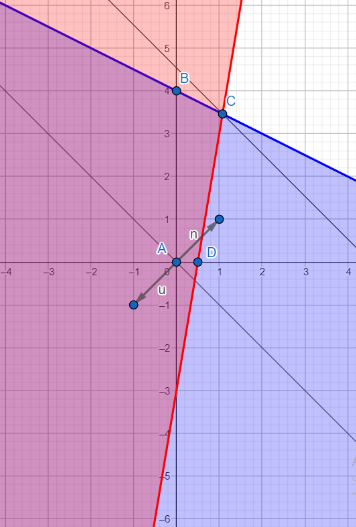
\includegraphics[]{пункт а.png}
\centering
\caption{График для решения задания №1, пункта 1a (построен с помощью \url{https://www.geogebra.org/calculator})}
\end{figure}

Без учета требования целочисленности:\\
Область допустимых значений - четырехугольник ABCD\\
$F_{max} = F(\frac{14}{13}; \frac{45}{13}) = \frac{59}{13}$
$x_1, x_2$ нецелочисленные\\

\begin{flushleft}
    {\bf2. Решение задачи симплекс методом} - см. №2а\\
\end{flushleft}

\begin{flushleft}
Приведем задачу к канонической форме:
\end{flushleft}

\begin{equation*}
    \begin{cases}
        x_1 + 2x_2 + x_3 = 8 \\
        6x_1 - x_2 + x_4 = 3 \\
        x_1, x_2 \in N_0, x_3, x_4 \ge 0
    \end{cases}
\end{equation*}

Оптимальная симплекс таблица без учета требования целочисленности:

\begin{center}
    \begin{tabular}{|c | c c c c c|} 
         \hline
            Базис & $x_1$ & $x_2$ & $x_3$ & $x_4$ & $b_i$\\
         \hline
            $x_2$ & 0 & 2 & $\frac{12}{13}$ & $-\frac{2}{13}$ & $\frac{90}{13}$\\
         \hline
            $x_1$ & 6.5 & 0 & 0.5 & 1 & 7\\
         \hline
            F(x) & 0 & 0 & $\frac{7}{13}$ & 1 & $\frac{59}{13}$\\
         \hline
    \end{tabular}
\end{center}

\begin{center}
    \begin{tabular}{|c | c c c c c|} 
         \hline
            Базис & $x_1$ & $x_2$ & $x_3$ & $x_4$ & $b_i$\\
         \hline
            $x_2$ & 0 & 1 & $\frac{6}{13}$ & $-\frac{1}{13}$ & $\frac{45}{13}$\\
         \hline
            $x_1$ & 1 & 0 & $\frac{1}{13}$ & $\frac{2}{13}$ & $\frac{14}{13}$\\
         \hline
            F(x) & 0 & 0 & $\frac{7}{13}$ & 1 & $\frac{59}{13}$\\
         \hline
    \end{tabular}
\end{center}

$F_{max} = F(\frac{14}{13}; \frac{45}{13}) = \frac{59}{13}$\\
$x_1, x_2$ нецелочисленные\\

\begin{flushleft}
    {\bf3. Решение задачи методом отсечения Гомори}\\
    {\bf3.1. Геометрическим методом}\\
\end{flushleft}

\begin{figure}[ht]
\centering
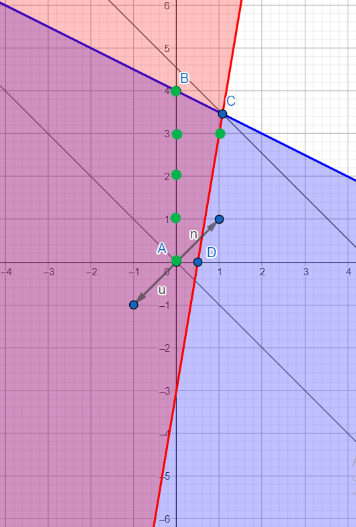
\includegraphics[]{пункт а_1.png}
\centering
\caption{График для решения ЗЦЛП (построен с помощью \url{https://www.geogebra.org/calculator})}
\end{figure}
Допустимые значения - множество зеленых точек\\
$\vec{n}\{1; 1\}$ - $\nabla F$ (градиент)\\
Если перемещать линию уровня (перпендикулярна $\vec{n}$) в направлении $\vec{n}$, то последняя точка, через которую пройдет линия, - точка с координатами (1; 3) - оптимальная точка\\
Значит $F_{max} = F(1; 3) = 1 + 3 = 4$\\
{\bfОтвет:~} $F_{max} = F(1; 3) = 4$

\begin{flushleft}
    {\bf3.2. Симплекс методом}\\
\end{flushleft}

Т.к. $\{\frac{45}{13}\} > \{\frac{14}{13}\}$, выпишем неравенство, соответствующее строке для $x_2$ в оптимальной симплекс таблице нецелочисленной задачи:\\
$\{0\} \cdot x_1 + \{1\} \cdot x_2 + \frac{6}{13} \cdot x_3 -\frac{1}{13} \cdot x_4 \ge \{\frac{45}{13}\}$\\
$\frac{6}{13} \cdot x_3 - \frac{1}{13} \cdot x_4 \ge \frac{6}{13}$\\
\begin{equation*}
    \begin{cases}
        6x_3 - x_4 \ge 6 \\
        x_3 = 8 - x_1 - 2x_2\\
        x_4 = 3 - 6x_1 + x_2\\
    \end{cases}
\end{equation*}
Значит:\\
$6\cdot (8 - x_1 - 2x_2) - (3 - 6x_1 + x_2) \ge 6$\\
$48 - 6x_1 - 12x_2 - 3 + 6x_1 - x_2 \ge 6$\\
$45 - 13x_2 \ge 6$\\
$x_1 \le 3$\\

Новая система ограничений:
\begin{equation*}
    \begin{cases}
        x_1 + 2x_2 \le 8 \\
        6x_1 - x_2 \le 3 \\
        x_2 \le 3\\
        x_1, x_2 \in N_0 
    \end{cases}
\end{equation*}

Каноническая форма:
\begin{equation*}
    \begin{cases}
        x_1 + 2x_2 + x_3 = 8 \\
        6x_1 - x_2 + x_4 = 3 \\
        x_2 + x_5 = 3\\
        x_1, x_2 \in N_0, x_3, x_4, x_5 \ge 0 
    \end{cases}
\end{equation*}

{\bf1-я симплекс-таблица:}

\begin{center}
    \begin{tabular}{|c | g c c c c c c|} 
         \hline
            Базис & $x_1$ & $x_2$ & $x_3$ & $x_4$ & $x_5$ & $b_i$ & $b_i/$р.с.\\
         \hline
            $x_3$ & 1 & 2 & 1 & 0 & 0 & 8 & 8/1 = 8\\
         \hline
         \rowcolor{LightBlue}
            $x_4$ & \cellcolor{cyan}6 & -1 & 0 & 1 & 0 & 3 & 3/6 = 1/2\\
         \hline
            $x_5$ & 0 & 1 & 0 & 0 & 1 & 3 & - \\
         \hline
            F(x) & -1 & -1 & 0 & 0 & 0 & 0 &\\
         \hline
    \end{tabular}
\end{center}

\begin{flushleft}
    Наименьшее значение в строке F(x): -1\\
    Разрешающий столбец: $x_1$\\
    Минимальное положительное значение из столбца $b_i$/р.с. : 1/2\\
    Разрешающий элемент: 6\\
    Не все значения в строке F(x) положительные $\implies$ решение не оптимально, строим новую таблицу\\
    {\bf2-я симплекс-таблица:}\\
\end{flushleft}

\begin{center}
    \begin{tabular}{|c | c g c c c c c|} 
         \hline
            Базис & $x_1$ & $x_2$ & $x_3$ & $x_4$ & $x_5$ & $b_i$ & $b_i/$р.с.\\
         \hline
            $x_3$ & 0 & $\frac{13}{6}$ & 1 & $-\frac{1}{6}$ & 0 & 7.5 & 7.5/($\frac{13}{6}$) = $\frac{45}{13}$\\
         \hline
            $x_1$ & 6 & -1 & 0 & 1 & 0 & 3 & 3/(-1) = -3\\
         \hline
         \rowcolor{LightBlue}
            $x_5$ & 0 & \cellcolor{cyan}1 & 0 & 0 & 1 & 3 & 3/1 = 3 \\
         \hline
            F(x) & 0 & $-\frac{7}{6}$ & 0 & $\frac{1}{6}$ & 0 & 0.5 &\\
         \hline
    \end{tabular}
\end{center}

\begin{flushleft}
    Наименьшее значение в строке F(x): $-\frac{7}{6}$\\
    Разрешающий столбец: $x_2$\\
    Минимальное положительное значение из столбца $b_i$/р.с. : 3\\
    Разрешающий элемент: $\frac{1}{6}$\\
    Не все значения в строке F(x) положительные $\implies$ решение не оптимально, строим новую таблицу\\
    {\bf3-я симплекс-таблица:}\\
\end{flushleft}

\begin{center}
    \begin{tabular}{|c | c c c c c c c|} 
         \hline
            Базис & $x_1$ & $x_2$ & $x_3$ & $x_4$ & $x_5$ & $b_i$ & $b_i/$р.с.\\
         \hline
            $x_3$ & 0 & 0 & 1 & $-\frac{1}{6}$ & $-\frac{13}{6}$ & 1 & \\
         \hline
            $x_1$ & 6 & 0 & 0 & 1 & 1 & 6 & \\
         \hline
            $x_2$ & 0 & 1 & 0 & 0 & 1 & 3 & \\
         \hline
            F(x) & 0 & 0 & 0 & $\frac{1}{6}$ & $\frac{7}{6}$ & 4 &\\
         \hline
    \end{tabular}
\end{center}

\begin{flushleft}
    Все значения в строке F(x) положительные, $F_{max} = 4$\\
    Оптимальное решение:\\
    $x_1 = 6/6 = 1$\\
    $x_2 = 3/1 = 3$\\
    $x_1, x_2$ целые $\implies$ задача целочисленного линейного программирования решена
\end{flushleft}

{\bfОтвет:~} $F_{max} = F(1; 3) = 4$
